
    \frame{
        \frametitle{Learning a linear ML model}


        \textbf{Setup:}\\[1em]
        \begin{itemize}
            \item Binary classification task $(X_i, y_i)_{i=1}^N \in \mathbb R^p \times \{-1, 1\}$
            \item Linear model: predict $y$ from $X$ with $\text{sign}(\langle \theta, X\rangle)$.
        \end{itemize}

        {\centering
        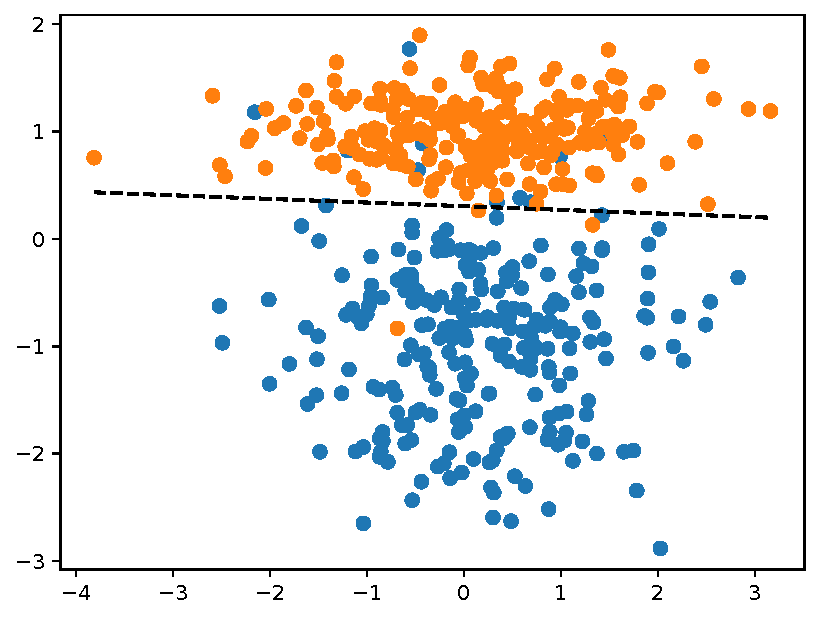
\includegraphics[width=.6\textwidth]{images/logreg_noreg}\\
        }

    }

    \frame{
        \frametitle{Learning a linear ML model}

        \textbf{Logistic loss:}\\[1em]

        \[
            G(\theta) = \frac1N \sum_{i=1}^N \log( 1 + e^{-y_i \langle \theta, X_i\rangle})
        \]


        \textbf{Training the model:}\\[1em]
        \[
            \theta^* = \argmin_\theta G(\theta)
        \]

    }

    \frame{
        \frametitle{Avoiding overfitting}

            Here, the second feature is uninformative,\\[2em]

            {\centering
            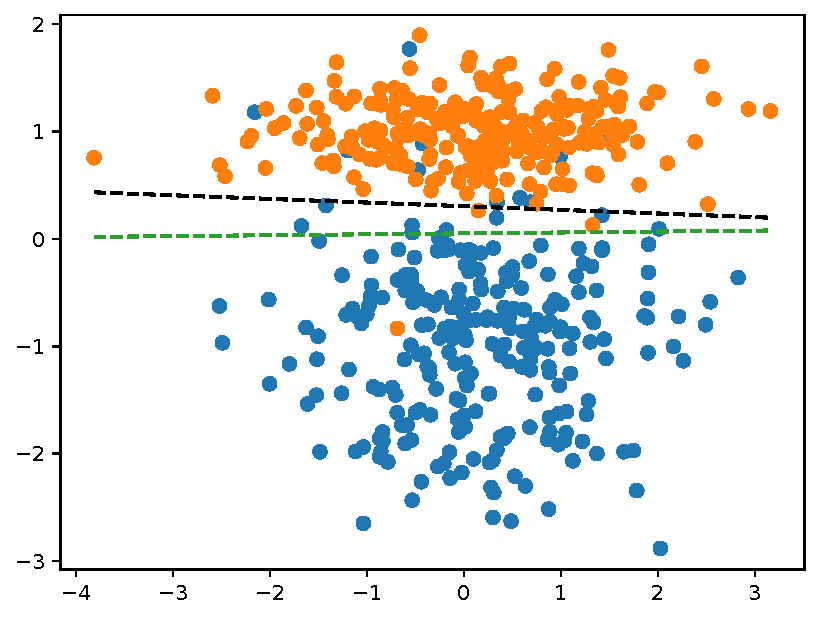
\includegraphics[width=.6\textwidth]{images/logreg_reg}\\
            }
    }
    \frame{
        \frametitle{Avoiding overfitting with a regularization}
        \textbf{\textcolor{blue!70}{Regularized} Logistic loss:}

        \[
            G(\theta, \lambda) = \frac1N \sum_{i=1}^N \log( 1 + e^{-y_i \langle \theta, X_i\rangle}) + \color{blue!70}\lambda\|\theta\|_2^2
        \]


        \textbf{Training the model:}\\[1em]
        \[
            \theta^*({\color{blue!70}\lambda}) = \argmin_\theta G(\theta,{\color{blue!70} \lambda})
        \]

        \pause
        \strongpoint{\bf \Large How to choose $\lambda$?}

    }

    \frame{
        \frametitle{Evaluating the generalization}

        We want to find $\lambda$ that ensure the best \emph{generalization} of $\theta^*(\lambda)$.\\[2em]

        \textbf{Validation loss:} use held out data $(X^{\it val}_i, y^{\it val}_i)_{i=1}^M$
        \[
            F(\theta) = \frac1M \sum_{i=1}^M \log( 1 + e^{-y^{\it val}_i \langle \theta, X_i^{\it val}\rangle})
        \]

        Independent estimate of the risk of the model.\\[1em]

        \pause
        \strongpoint{Find $\lambda$ that gives a model $\theta^*(\lambda)$ with a good validation loss.}
    }

    \frame{
        \frametitle{The Grid Search}

        \begin{itemize}\itemsep1.5em
            \item Select a grid of parameters $\{\lambda_1,\dots \lambda_K\}$.
            \item Train a model for each parameter $\lambda_k$: $\theta^*(\lambda_k)$.
            \item Evaluate the performance with the validation loss $F(\theta^*(\lambda_k))$.
            \item Keep the value $\lambda_k$ with the best performance.
        \end{itemize}

        \pause
        \vskip2em
        \textbf{Mathematical rewritting:}
        \[\begin{cases}
            \quad\min_{\lambda \in \{\lambda_1,\dots \lambda_K\}}
            F(\theta^*(\lambda))\\
            s.t.\quad \theta^*(\lambda) = \argmin_\theta G(\theta, \lambda)
        \end{cases}\]
    }

    \frame{
        \frametitle{The Grid Search with multiple hyperparameters}

        \textbf{Regularized Logistic loss:}

        \[
            G(\theta, \lambda) = \frac1N \sum_{i=1}^N \log( 1 + e^{-y_i \langle \theta, X_i\rangle}) + \alt<2->{\color{blue!70}\sum_{k=1}^p\lambda_k\theta_k^2}{\lambda\|\theta\|_2^2}
        \]

        \visible<2->{
            Grid search is inefficient as the grid increases exponentially with the number of parameters.
        }
        \vskip2em

        \visible<3>{
            \strongpoint{\bf\large Can we use first-order methods to minimize $h(\lambda) = F(\theta^*(\lambda))$?}
        }
    }